%% The following is a directive for TeXShop to indicate the main file
%%!TEX root = diss.tex

\chapter{Materials and Methods}
\label{ch:Materialsandmethods}

%%%%%%%%%%%%%%%%%%%%%%%%%%%%%%%%%%%%%%%%%%%%%%%%%%%%%%%%%%%%%%%%%%%%%%
\section{Patient Samples}
\label{sec:PatientSamples}

Solid tumour biopsies were collected from 171 consented patients in The Oncopanel Pilot (TOP) study under a protocol approved by the British Columbia Cancer Agency (BCCA) Research Ethics Board (Protocol H12-00292). Details on tumour types are listed in \autoref{tbl:FFPE:Specimen}. Excess tissue from tumuor biopsies after pathological evaluation were transported in serum-free medium at ambient temperature followed by washing in PBS with 6.5mM dithiothreitol (DTT). Fat, muscle, and necrotic areas were trimmed and approximately 50-100 mg of specimens were formalin-fixed at 4$^{\circ}$C overnight before paraffin-embedding. All specimens were fixed within 2 hours and embedded within 24 hours of collection. For each patient in the TOP cohort, peripheral blood (PB) samples were also collected and processed to serve as germline DNA control for variant calling.

\begin{table}[!htb]
    \caption{Summary of FFPE Specimens from 171 TOP Patients}
    \label{tbl:FFPE:Specimen}
    \centering
    \begin{tabular}{ l c c }\toprule
    Tumour Type & Number of Specimens & Percentage \\
    \midrule
    Colorectal & 85 & 49.7 \\
    Lung & 36 & 21.1 \\
    Melanoma & 16 & 9.4 \\
    Other & 30 & 17.5 \\
    Unknown & 6 & 3.5 \\
    \bottomrule
    \end{tabular}
\end{table}

%%%%%%%%%%%%%%%%%%%%%%%%%%%%%%%%%%%%%%%%%%%%%%%%%%%%%%%%%%%%%%%%%%%%%%
\section{DNA Extraction, Library Preparation, and Illumina Sequencing}
\label{sec:DNAExtraction}

Tumour and germline DNA for 171 patients were extracted using the QIAGEN FFPE DNA extraction kit and xx respectively as per manufacturer's instructions. For specimens with sufficient DNA quantity, 250 ng of genomic DNA was used for library preparation. Genomic DNA was sheared to generate fragment sizes of approximately 3 kbp, followed by PCR primer merging, amplicon generation, and adapter ligation using the RainDance Thunderstorm instrument (\autoref{fig:lib-prep-workflow}). The complete list of primers used to generate the 429 amplicons for 26 genes screened by the OncoPanel is included in \autoref{tbl:amplicon:list}. Six out of 26 genes are PGx genes namely \textit{DPYD}, \textit{GSTP1}, \textit{MTHFR}, \textit{TYMP}, \textit{TYMS}, and \textit{UGT1A1}. Libraries were pooled, ranging from 13-20 libraries per pool, and sequenced with the Illumina MiSeq system for paired end sequencing with a v2 250-bp kit. Pooling of libraries includes libraries from other studies, which is summarized in \autoref{fig:lib-pooling}.

\begin{figure}
    \centering
    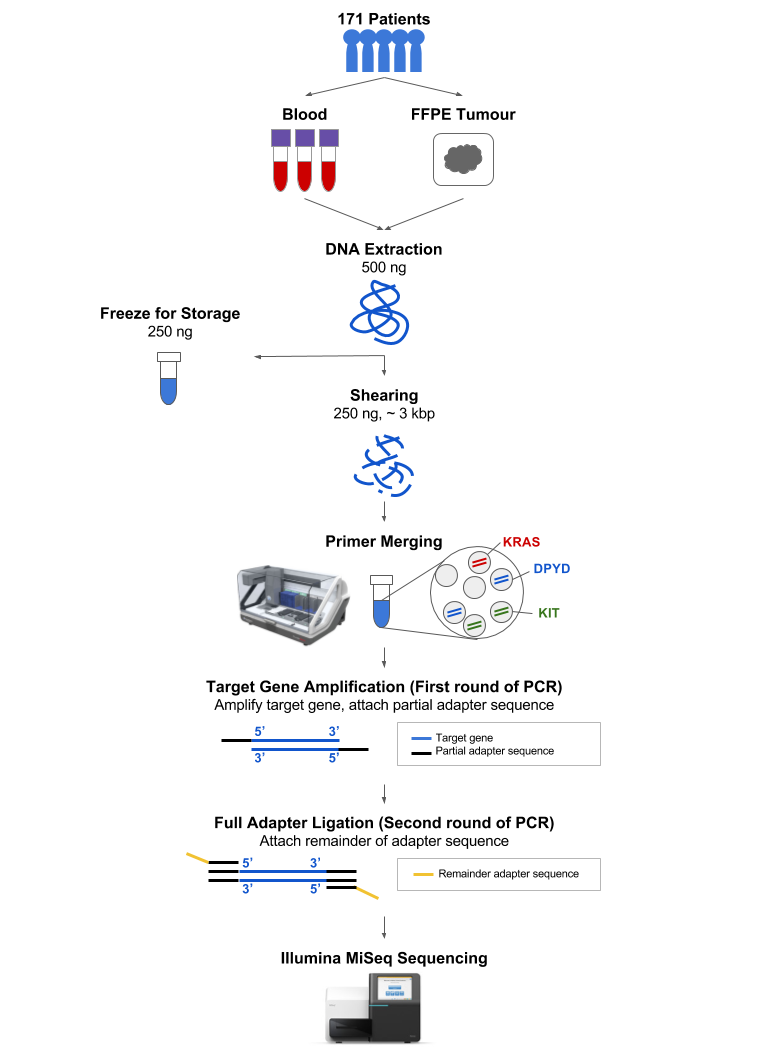
\includegraphics[width=5.5in, height=8in]{/Users/evayap/Documents/masters_thesis/ubcdiss/mm_figures/lib_prep_workflow.png}
    \caption{Workflow for Sample Processing, Library Preparation, and NGS Sequencing.}
    \label{fig:lib-prep-workflow}   % label should change
\end{figure}

\begin{figure}
    \centering
    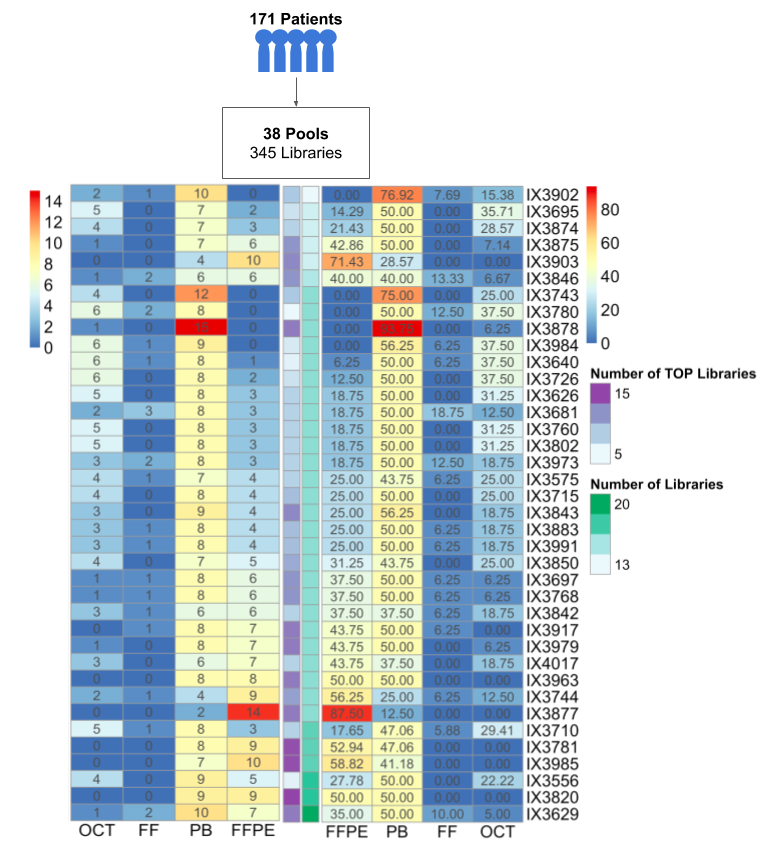
\includegraphics[width=7in, height=8in]{/Users/evayap/Documents/masters_thesis/ubcdiss/mm_figures/lib_pool.png}
    \caption{345 TOP Libraries Distributed Across 38 Pools. Number of libraries is presented on the \textit{left} whereas percentage of libraries per total libraries in a pool is presented on the \textit{right}.}
    \label{fig:lib-pooling}   % label should change
\end{figure}

%%%%%%%%%%%%%%%%%%%%%%%%%%%%%%%%%%%%%%%%%%%%%%%%%%%%%%%%%%%%%%%%%%%%%%
\section{Variant Calling Pipeline}
\label{sec:VariantCallingPipeline}

Read alignment and variant calling were carried out by the BCCA Centre of Clinical Genomics (CCG) bioinformatics pipeline \autoref{fig:ccg-pipeline}. Raw reads from the MiSeq instrument were aligned to the GRCh37 human reference genome (hg19) using BWA (version 0.5.9, mem algorithm) and variant calling was performed using samtools mpileup (version 0.1.18) followed by VarScan2 (version 2.3.6). Variant calling in the six PGx genes were carried out using the following VarScan2 parameters: Variants were annotated as per the Human Genome Variation Society (HGVS) convention and interpreted with databases such as dbSNP, ExAC, COSMIC, and ClinVar using SnpEff (version 4.2). Gene reference models used for HGVS nomenclature are listed in \autoref{tbl:HGVS:gene:model}.

\begin{figure}
    \centering
    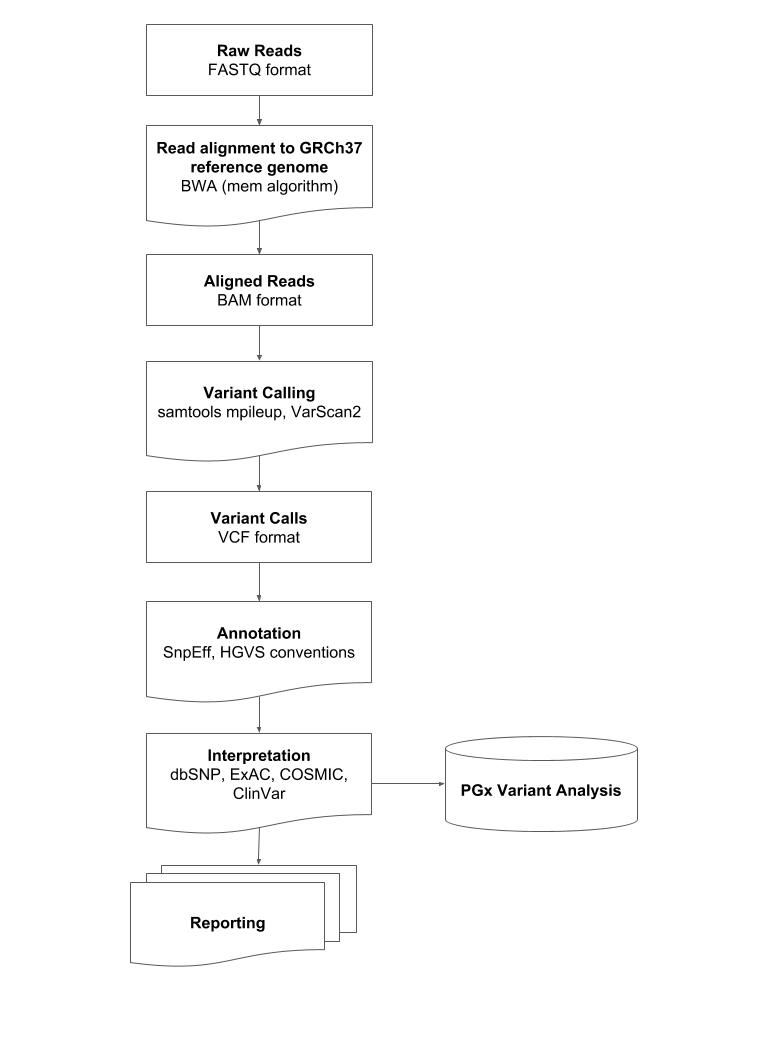
\includegraphics[width=5.5in, height=8in]{/Users/evayap/Documents/masters_thesis/ubcdiss/mm_figures/variant_calling.png}
    \caption{OncoPanel Pipeline for Variant Calling. Variants in PGx genes were filtered for downstream analysis.}
    \label{fig:ccg-pipeline}   % label should change
\end{figure}

%%%%%%%%%%%%%%%%%%%%%%%%%%%%%%%%%%%%%%%%%%%%%%%%%%%%%%%%%%%%%%%%%%%%%%
\section{Data Analysis and Visualization}
\label{sec:DataAnalysisandVisualization}

Coverage depth was measured using bedtools (version 2.25.0) and per-base metrics were obtained using bam-readcount (https://github.com/genome/). Statistical analyses and data visualization were performed using R (version 3.3.2) and associated open-source packages. Manual review of PGx variants were carried out using the Intergrative Genomics Viewer (IGV, version 2.3). \textit{Note: be more specific on how the data is generated}

\endinput
%%%%%%%%%%%%%%%%%%%%%%%%%%%%%%%%%%%%%%%%%%%%%%%%%%%%%%%%%%%%%%%%%%%%%%
\section{Introduction}
\label{sec:Introduction}

Genomics-driven oncology is an emerging approach that aims to use genomic information for patient management and therapeutic intervention in oncologic care. Using MPS technologies, cancer biomarkers with diagnostic, prognostic, predictive, and pharmacogenomic (PGx) significance can be screened at a reduced cost and turn-around time to inform medical decision-making. PGx markers are germline genetic

Application of genome information to guide patient management and therapeutic intervention holds great potential in improving oncology care. One of the driving forces that led to clinical feasibility of genomic sequencing is the advent of massively parallel sequencing (MPS) technologies, which enabled sensitive and accurate sequencing of more target genes with less DNA in a cost-effective and timely manner. At present, various MPS approaches are entering, or have entered the clinic such as targeted sequencing panels, whole exome sequencing, and whole genome sequencing, which create the opportunity to further develop novel clinical biomarkers in addition to screening for biomarkers with established clinical utility.

In the context of cancer,
Clinical biomarkers can be classified as diagnostic, prognostic, predictive, and pharmacogenomic (PGx). In the context of cancer, both somatic Germline variants that affect influence drug response are PGx biomarkers.

In the context of cancer, PGx biomarkers are

Clinical molecular laboratories are rapidly adopting and leveraging the advances in massively parallel sequencing (MPS) technologies for germline and tumour profiling. have driven the clinical use of genomic information to guide patient management and therapeutic intervention in oncology care. The ability of MPS to sensitively and accurately sequence more target genes with less DNA in a cost-effective and timely manner perfectly meet the clinical reality which is to do more with less.

reduced cost, time and labor high throughput nature, decreased sequencing cost, and increased sensitivity, and ability to Genomics-driven cancer medicine aims is driven by the advances in massively parallel sequencing (MPS) technologies, the reduced cost of genome sequencing, and development of bioinformatics analytic tools. This emerging framework in the oncology care aims to use genomics information to inform

The Oncopanel is a clinical targeted sequencing panel for solid tumours provided by the CCG at the BCCA. In addition to somatic mutations, it screens for germline variants in PGx genes such as DPYD, GSTP1, MTHFR, TYMP, TYMS, and UGT1A1 (Table 1). Detection of germline PGx variants is essential for chemotherapy selection and optimization of treatment dosage and duration. The Oncopanel is also delivered as a single sample clinical assay in which genetic variants are detected in DNA from FFPE tumours. However, formalin fixation causes DNA fragmentation and base transition artifacts (i.e. C$>$T and G$>$A). Hence, I investigated whether germline PGx variants could be detected with high sensitivity and precision in FFPE tumour DNA compared to blood DNA which is the gold standard for germline variant calling.
